\documentclass{beamer}
\usetheme[sectionpage=progressbar, subsectionpage=progressbar, numbering=fraction, progressbar=foot, block=fill, background=light]{metropolis}
\usepackage{appendixnumberbeamer}
\usepackage{textpos}
\usepackage{booktabs}
\usepackage[scale=2]{ccicons}

\usepackage{pgfplots}
\usepgfplotslibrary{dateplot}
\usetikzlibrary{backgrounds}
\usepackage{xspace}
\newcommand{\themename}{\textbf{\textsc{metropolis}}\xspace}
\title{Attention based models in End-to-End ASR}
\subtitle{Exploration of Attention in ESPNET toolkit}
\date{\today}
\author{Shreekantha Nadig}
\institute{International Institute of Information Technology - Bangalore}
%\titlegraphic{\hfill\includegraphics[height=1.5cm]{logo.pdf}}

\usepackage{tikz}
\usetikzlibrary{shapes,shadows,arrows,patterns, matrix, calc}

\tikzstyle{line} = [draw, -latex']
\tikzstyle{round} = [draw, circle, fill=black!30, minimum size=4em, node distance=4em, font=\fontsize{30}{10}\selectfont]
\tikzstyle{mlp_enc} = [rectangle, draw, fill=red!50, text width=2cm, minimum height=5em, text centered, node distance=10em, font=\fontsize{20}{10}\selectfont]
\tikzstyle{mlp_att} = [rectangle, draw, fill=green!50, text width=2cm, minimum height=5em, text centered, node distance=10em, font=\fontsize{20}{10}\selectfont]
\tikzstyle{mlp_dec} = [rectangle, draw, fill=blue!50, text width=2cm, minimum height=5em, text centered, node distance=10em, font=\fontsize{20}{10}\selectfont]
\tikzstyle{enc_h} = [rectangle, draw,  pattern=horizontal lines, pattern color=red!60, text width=1cm, minimum height=10em, minimum width=3em, text centered, node distance=10em, font=\fontsize{25}{10}\selectfont]
\tikzstyle{atts} = [rectangle, draw,  pattern=horizontal lines, pattern color=green!70, text width=1cm, minimum height=10em, minimum width=3em, text centered, node distance=10em, font=\fontsize{20}{10}\selectfont]
\tikzstyle{dec_z} = [rectangle, draw,  pattern=horizontal lines, pattern color=blue!60, text width=1cm, minimum height=10em, minimum width=3em, text centered, node distance=10em, font=\fontsize{20}{10}\selectfont]
\tikzstyle{cnn} = [rectangle, draw,  pattern=crosshatch, pattern color=red!50!blue!50, text width=2cm, minimum height=5em, text centered, node distance=10em, font=\fontsize{20}{10}\selectfont]
\tikzstyle{box} = [rectangle, draw,  fill=blue!20, text width=3cm, minimum height=5em, minimum width=3em, text centered, node distance=10em, font=\fontsize{20}{10}\selectfont]

\pgfdeclarelayer{background}
\pgfdeclarelayer{foreground}
\pgfsetlayers{background,main,foreground}

\begin{document}
	\addtobeamertemplate{frametitle}{}{%
		\begin{textblock*}{100mm}(.97\textwidth,-1cm)
			{
\includegraphics[width=2.5em]{iiitb_logo.png}}
		\end{textblock*}}

%\maketitle
\section{MultiHead Attention}
\begin{frame}[fragile]{Attention Is All You Need}
	\begin{itemize}
		\item Most competitive neural sequence transduction models have an encoder-decoder structure [1]
		\item Transformer : Solely based on Attention (No Recurrent / Convolutional connections)
		\item Recurrent model : Can't parallelize within an example
		\item Attention is almost always used with Recurrent Networks (before)
		\item Transformer : Relying entirely on Attention
		\item Self Attention / Intra Attention
	\end{itemize}
[1] D. Bahdanau, K. Cho, and Y. Bengio, “Neural Machine Translation by Jointly Learning to Align and Translate,” Sep. 2014.
\end{frame}

\begin{frame}[fragile]{Attention Is All You Need - Important topics}
\begin{itemize}
	\item Self Attention / Intra Attention
	\item Scaled Dot Product Attention
	\item Mutli-Head Attention
	\item Attention - K,V and Q
	\item Position wise FeedForward Networks
	\item Positional Encoding
	\item Residual Connections
	\item Learning rate scheduling
\end{itemize}
\end{frame}


\begin{frame}[fragile]{Attention}
\begin{block}{Attention}
	An attention function can be described as mapping a query and a set of key-value pairs to an output.
\end{block}

\begin{itemize}
	\item The \textcolor{green}{query}, \textcolor{red!60}{keys}, \textcolor{red}{values}, and output are all vectors
	\item  The output is computed as a weighted sum of the values, where the weight assigned to each value is computed by a compatibility function of the query with the corresponding key.
	\item Query : $dec_z \in \mathcal{R}^{d_k}$
	\item Key : $f(h) \in \mathcal{R}^{d_k}$
	\item Value : $g(h) \in \mathcal{R}^(d_v)$
	\item $Attention(Q,K,V) = Softmax(\dfrac{QK^T}{\sqrt{d_k}}) V$
\end{itemize}
\end{frame}

\begin{frame}[fragile]{Scaled Dot product}
\begin{center}
	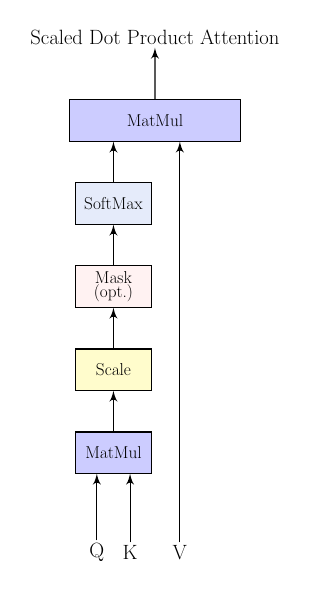
\begin{tikzpicture}[scale=0.3, every node/.style={transform shape, font=\fontsize{40}{40}\selectfont}]
	
	\node [box] (mm1) {MatMul};
	\node [box, above of = mm1, fill=yellow!20] (scale1) {Scale};
	\node [box, above of = scale1, fill=pink!20] (mask) {Mask (opt.)};
	\node [box, above of = mask, fill=green!20!blue!10] (sm) {SoftMax};
	\node [box, above of = sm, xshift = 5em, text width = 20em] (mm2) {MatMul};
	\node [below of=mm1, node distance = 12em, xshift = -2em] (q) {Q};
	\node [below of=mm1, node distance = 12em, xshift = 2em] (k) {K};
	\node [below of=mm1, node distance = 12em, xshift = 8em] (v) {V};
	
	\path [line] (k.north) -- (k.north |- mm1.south);
	\path [line] (q.north) -- (q.north |- mm1.south);
	\path [line] (v.north) -- (v.north |- mm2.south);
	
	\path [line] (mm1.north) to (scale1.south);
	\path [line] (scale1.north) to (mask.south);
	\path [line] (mask.north) to (sm.south);
	\path [line] (sm.north) -- (sm.north |- mm2.south);
	
	\node [above of = mm2, node distance = 10em] (e) {Scaled Dot Product Attention};
	\path [line] (mm2.north) to (e.south);
	\end{tikzpicture}
\end{center}
\end{frame}


\begin{frame}[fragile]{Scaled Dot Product}
	$$Attention(Q,K,V) = Softmax(\dfrac{QK^T}{\sqrt{d_k}}) V$$
	\begin{itemize}
		\item compute the dot products of the query with all keys
		\item divide each by $\sqrt{d_k}$
		\item apply a softmax function to obtain the weights on the values
	\end{itemize}
	
	\begin{block}{Dot Product Attention}
		Dot Product Attention is similar to this except for the scaling factor $1 / \sqrt{d_k}$
	\end{block}
	
	\begin{itemize}
		\item For large dk AttAdd > MultiHeadDot [3]
		\item The dot products grow large in magnitude, pushing the softmax function into regions where it has extremely small gradients -> Scale the dot product
	\end{itemize}
[3] D. Britz, A. Goldie, M.-T. Luong, and Q. Le, “Massive Exploration of Neural Machine Translation Architectures,” Mar. 2017.
\end{frame}

\begin{frame}[fragile]{Multi-Head Attention}
\begin{center}
	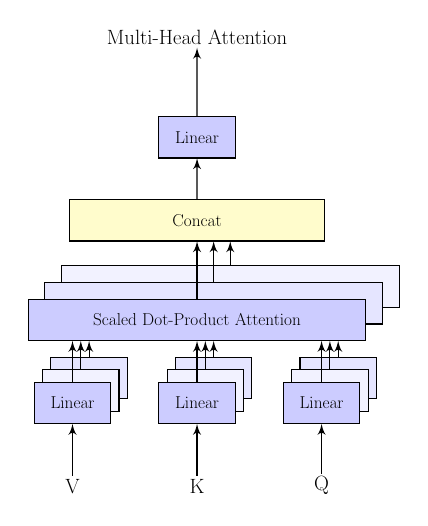
\begin{tikzpicture}[scale=0.3, every node/.style={transform shape, font=\fontsize{40}{40}\selectfont}]
	
	\node [box] (lin1) {Linear};
	\node [box, right of=lin1, node distance = 15em] (lin2) {Linear};
	\node [box, right of=lin2, node distance = 15em] (lin3) {Linear};
	
	\node [box, above of = lin2, text width = 40em] (sd1) {Scaled Dot-Product Attention};
	
	\begin{scope}[on background layer]
	\node [box, above of = lin1, node distance = 3em, fill=blue!10, xshift=2em, fill=blue!10] (lin22)
	{};
	\node [box, above of = lin1, node distance = 1.5em, fill=blue!10, xshift=1em, fill=blue!5] (lin21)
	{};
	
	\node [box, above of = lin2, node distance = 3em, fill=blue!10, xshift=2em, fill=blue!10] (lin32)
	{};
	\node [box, above of = lin2, node distance = 1.5em, fill=blue!10, xshift=1em, fill=blue!5] (lin31)
	{};
	
	\node [box, above of = lin3, node distance = 3em, fill=blue!10, xshift=2em, fill=blue!10] (lin42)
	{};
	\node [box, above of = lin3, node distance = 1.5em, fill=blue!10, xshift=1em, fill=blue!5] (lin41)
	{};
	
	\node [box, above of = sd1, text width = 40em, node distance = 4em, xshift = 4em, fill=blue!5] (sd3) {};
	\node [box, above of = sd1, text width = 40em, node distance = 2em, xshift = 2em, fill=blue!10] (sd2) {};
	\end{scope}
	
	\path [line] (lin1.north) -- (lin1.north |- sd1.south);
	\path [line] (lin2.north) -- (lin2.north |- sd1.south);
	\path [line] (lin3.north) -- (lin3.north |- sd1.south);
	
	\path [line] (lin22.north) -- (lin22.north |- sd1.south);
	\path [line] (lin32.north) -- (lin32.north |- sd1.south);
	\path [line] (lin42.north) -- (lin42.north |- sd1.south);
	
	\path [line] (lin21.north) -- (lin21.north |- sd1.south);
	\path [line] (lin31.north) -- (lin31.north |- sd1.south);
	\path [line] (lin41.north) -- (lin41.north |- sd1.south);
	
	\node [box, above of = sd1, node distance = 12em, fill=yellow!20, text width = 30em] (concat) {Concat};
	\node [box, above of = concat] (linear) {Linear};
	
	\path [line] (sd1.north) -- (sd1.north |- concat.south);
	\path [line] (sd2.north) -- (sd2.north |- concat.south);
	\path [line] (sd3.north) -- (sd3.north |- concat.south);
	\path [line] (concat.north) to (linear.south);
	
	\node [above of = linear, node distance = 12em] (mh) {Multi-Head Attention};
	\path [line] (linear.north) to (mh.south);
	
	\node [below of=lin1, node distance = 10em] (V) {V};
	\node [below of=lin2, node distance = 10em] (K) {K};
	\node [below of=lin3, node distance = 10em] (Q) {Q};
	
	\path [line] (V.north) -- (V.north |- lin1.south);
	\path [line] (K.north) -- (K.north |- lin2.south);
	\path [line] (Q.north) -- (Q.north |- lin3.south);
	
	\end{tikzpicture}
\end{center}
\end{frame}


\begin{frame}[fragile]{Multi Head Attention}
Instead of a Single Attention with Q, K, V :
\begin{itemize}
	\item Linearly Project Q,K,V to $d_k, d_k, d_v$ dimensions - h times!
	\item Perform Attention on each of these Q,K,V in parallel to yield $d_v$ dimensional values
	\item $d_{v}^{i}$ where $i = 1 \dots h$
	\item All are concatenated and projected to get the final value
\end{itemize}
	\begin{block}{Advantage over Single Head attention}
		This allows the model to jointly attend to information from different representation at different positions
	\end{block}
	\begin{alertblock}{Single Head Attention}
		Averaging inhibits this behavior
	\end{alertblock}
\end{frame}

\begin{frame}[fragile]{Projections of Q,K,V}
	\begin{itemize}
		\item $W_{i}^{Q} \in \mathcal{R}^{d_{model} \times d_{k}}$
		\item $W_{i}^{K} \in \mathcal{R}^{d_{model} \times d_{k}}$
		\item $W_{i}^{V} \in \mathcal{R}^{d_{model} \times d_{v}}$
		\item $W_{i}^{O} \in \mathcal{R}^{hd_{v} \times d_{model}}$
		\item Here, h=8 parallel attention layers or heads
		\item $d_k = d_v = d_{model}/h = 64$
	\end{itemize}
	
	\begin{block}{Computational Cost}
		Due to the reduced dimension of each head, the total computational cost is similar to that of single-head attention with full dimensionality.
	\end{block}
\end{frame}







\begin{frame}[fragile]{MultiHead Dot Product Attention - Full picture}
\begin{center}
	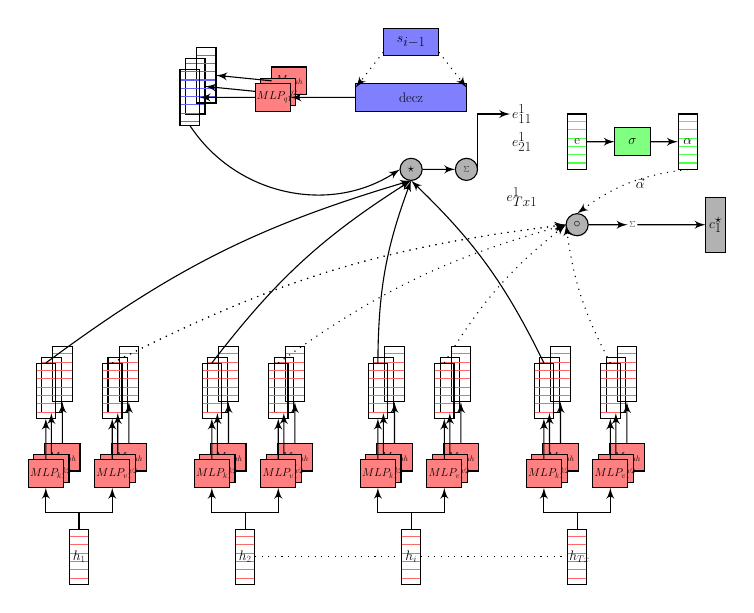
\begin{tikzpicture}[scale=0.2, every node/.style={transform shape, font=\fontsize{40}{40}\selectfont}]
	
	\node [enc_h] (h1) {$h_{1}$};
	\node [enc_h,right of = h1, node distance = 30em] (h2) {$h_{2}$};
	\node [enc_h,right of = h2, node distance = 30em] (hi) {$h_{i}$};
	\node [enc_h,right of = hi, node distance = 30em] (hTx) {$h_{Tx}$};
	\draw [dotted] (h2.east) to (hi.west);
	\draw [dotted] (hi.east) to (hTx.west);
	
	\begin{pgfonlayer}{foreground}
	\node [mlp_enc, above of=h1, xshift=-6em, node distance = 15em] (mlpk11) {$MLP_{k1}$};
	\end{pgfonlayer}	
	
	\begin{pgfonlayer}{main}
	\node [mlp_enc, above of=mlpk11, node distance = 1em, xshift=1em] (mlpk21) {$MLP_{k2}$};
	\end{pgfonlayer}
	
	\begin{pgfonlayer}{background}
	\node [mlp_enc, above of=mlpk21, node distance = 2em, xshift=2em] (mlpk31) {$M_{k\_ah}$};
	\end{pgfonlayer}
	
	
	
	\begin{pgfonlayer}{foreground}
	\node [mlp_enc, above of=h1, xshift=6em, node distance = 15em] (mlpv11) {$MLP_{v1}$};
	\end{pgfonlayer}	
	
	\begin{pgfonlayer}{main}
	\node [mlp_enc, above of=mlpv11, node distance = 1em, xshift=1em] (mlpv21) {$MLP_{v2}$};
	\end{pgfonlayer}
	
	\begin{pgfonlayer}{background}
	\node [mlp_enc, above of=mlpv21, node distance = 2em, xshift=2em] (mlpv31) {$M_{v\_ah}$};
	\end{pgfonlayer}
	
	\path [line] (h1.north) -- ($(h1.north) - (0,-3em)$) -| (mlpk11.south);
	\path [line] (h1.north) -- ($(h1.north) - (0,-3em)$) -| (mlpv11.south);
	
	
	
	\begin{pgfonlayer}{foreground}
	\node [mlp_enc, above of=h2, xshift=-6em, node distance = 15em] (mlpk12) {$MLP_{k1}$};
	\end{pgfonlayer}	
	
	\begin{pgfonlayer}{main}
	\node [mlp_enc, above of=mlpk12, node distance = 1em, xshift=1em] (mlpk22) {$MLP_{k2}$};
	\end{pgfonlayer}
	
	\begin{pgfonlayer}{background}
	\node [mlp_enc, above of=mlpk22, node distance = 2em, xshift=2em] (mlpk32) {$M_{k\_ah}$};
	\end{pgfonlayer}
	
	
	
	\begin{pgfonlayer}{foreground}
	\node [mlp_enc, above of=h2, xshift=6em, node distance = 15em] (mlpv12) {$MLP_{v1}$};
	\end{pgfonlayer}	
	
	\begin{pgfonlayer}{main}
	\node [mlp_enc, above of=mlpv12, node distance = 1em, xshift=1em] (mlpv22) {$MLP_{v2}$};
	\end{pgfonlayer}
	
	\begin{pgfonlayer}{background}
	\node [mlp_enc, above of=mlpv22, node distance = 2em, xshift=2em] (mlpv32) {$M_{v\_ah}$};
	\end{pgfonlayer}
	
	\path [line] (h2.north) -- ($(h2.north) - (0,-3em)$) -| (mlpk12.south);
	\path [line] (h2.north) -- ($(h2.north) - (0,-3em)$) -| (mlpv12.south);
	
	
	\begin{pgfonlayer}{foreground}
	\node [mlp_enc, above of=hi, xshift=-6em, node distance = 15em] (mlpk13) {$MLP_{k1}$};
	\end{pgfonlayer}	
	
	\begin{pgfonlayer}{main}
	\node [mlp_enc, above of=mlpk13, node distance = 1em, xshift=1em] (mlpk23) {$MLP_{k2}$};
	\end{pgfonlayer}
	
	\begin{pgfonlayer}{background}
	\node [mlp_enc, above of=mlpk23, node distance = 2em, xshift=2em] (mlpk33) {$M_{k\_ah}$};
	\end{pgfonlayer}
	
	
	
	\begin{pgfonlayer}{foreground}
	\node [mlp_enc, above of=hi, xshift=6em, node distance = 15em] (mlpv13) {$MLP_{v1}$};
	\end{pgfonlayer}	
	
	\begin{pgfonlayer}{main}
	\node [mlp_enc, above of=mlpv13, node distance = 1em, xshift=1em] (mlpv23) {$MLP_{v2}$};
	\end{pgfonlayer}
	
	\begin{pgfonlayer}{background}
	\node [mlp_enc, above of=mlpv23, node distance = 2em, xshift=2em] (mlpv33) {$M_{v\_ah}$};
	\end{pgfonlayer}
	
	\path [line] (hi.north) -- ($(hi.north) - (0,-3em)$) -| (mlpk13.south);
	\path [line] (hi.north) -- ($(hi.north) - (0,-3em)$) -| (mlpv13.south);
	
	
	
	\begin{pgfonlayer}{foreground}
	\node [mlp_enc, above of=hTx, xshift=-6em, node distance = 15em] (mlpk14) {$MLP_{k1}$};
	\end{pgfonlayer}	
	
	\begin{pgfonlayer}{main}
	\node [mlp_enc, above of=mlpk14, node distance = 1em, xshift=1em] (mlpk24) {$MLP_{k2}$};
	\end{pgfonlayer}
	
	\begin{pgfonlayer}{background}
	\node [mlp_enc, above of=mlpk24, node distance = 2em, xshift=2em] (mlpk34) {$M_{k\_ah}$};
	\end{pgfonlayer}
	
	
	
	\begin{pgfonlayer}{foreground}
	\node [mlp_enc, above of=hTx, xshift=6em, node distance = 15em] (mlpv14) {$MLP_{v1}$};
	\end{pgfonlayer}	
	
	\begin{pgfonlayer}{main}
	\node [mlp_enc, above of=mlpv14, node distance = 1em, xshift=1em] (mlpv24) {$MLP_{v2}$};
	\end{pgfonlayer}
	
	\begin{pgfonlayer}{background}
	\node [mlp_enc, above of=mlpv24, node distance = 2em, xshift=2em] (mlpv34) {$M_{v\_ah}$};
	\end{pgfonlayer}
	
	\path [line] (hTx.north) -- ($(hTx.north) - (0,-3em)$) -| (mlpk14.south);
	\path [line] (hTx.north) -- ($(hTx.north) - (0,-3em)$) -| (mlpv14.south);
	
	
	\begin{pgfonlayer}{foreground}
	\node [enc_h, above of= mlpk11, node distance = 15em] (k11) {};
	\end{pgfonlayer}	
	
	\begin{pgfonlayer}{main}
	\node [enc_h, above of= mlpk21,node distance = 15em] (k21) {};
	\end{pgfonlayer}
	
	\begin{pgfonlayer}{main}
	\node [enc_h, above of= mlpk31, node distance = 15em] (k31) {};
	\end{pgfonlayer}
	
	
	\begin{pgfonlayer}{foreground}
	\node [enc_h, above of= mlpv11, node distance = 15em] (v11) {};
	\end{pgfonlayer}	
	
	\begin{pgfonlayer}{main}
	\node [enc_h, above of= mlpv21,node distance = 15em] (v21) {};
	\end{pgfonlayer}
	
	\begin{pgfonlayer}{main}
	\node [enc_h, above of= mlpv31, node distance = 15em] (v31) {};
	\end{pgfonlayer}
	
	
	\path [line] (mlpk31.north) to (k31.south); 
	\path [line] (mlpk21.north) to (k21.south); 
	\path [line] (mlpk11.north) to (k11.south); 
	
	\path [line] (mlpv31.north) to (v31.south); 
	\path [line] (mlpv21.north) to (v21.south); 
	\path [line] (mlpv11.north) to (v11.south); 
	
	
	\begin{pgfonlayer}{foreground}
	\node [enc_h, above of= mlpk12, node distance = 15em] (k12) {};
	\end{pgfonlayer}	
	
	\begin{pgfonlayer}{main}
	\node [enc_h, above of= mlpk22,node distance = 15em] (k22) {};
	\end{pgfonlayer}
	
	\begin{pgfonlayer}{main}
	\node [enc_h, above of= mlpk32, node distance = 15em] (k32) {};
	\end{pgfonlayer}
	
	
	\begin{pgfonlayer}{foreground}
	\node [enc_h, above of= mlpv12, node distance = 15em] (v12) {};
	\end{pgfonlayer}	
	
	\begin{pgfonlayer}{main}
	\node [enc_h, above of= mlpv22,node distance = 15em] (v22) {};
	\end{pgfonlayer}
	
	\begin{pgfonlayer}{main}
	\node [enc_h, above of= mlpv32, node distance = 15em] (v32) {};
	\end{pgfonlayer}
	
	
	\path [line] (mlpk32.north) to (k32.south); 
	\path [line] (mlpk22.north) to (k22.south); 
	\path [line] (mlpk12.north) to (k12.south); 
	
	\path [line] (mlpv32.north) to (v32.south); 
	\path [line] (mlpv22.north) to (v22.south); 
	\path [line] (mlpv12.north) to (v12.south); 
	
	
	
	\begin{pgfonlayer}{foreground}
	\node [enc_h, above of= mlpk13, node distance = 15em] (k13) {};
	\end{pgfonlayer}	
	
	\begin{pgfonlayer}{main}
	\node [enc_h, above of= mlpk23,node distance = 15em] (k23) {};
	\end{pgfonlayer}
	
	\begin{pgfonlayer}{main}
	\node [enc_h, above of= mlpk33, node distance = 15em] (k33) {};
	\end{pgfonlayer}
	
	
	\begin{pgfonlayer}{foreground}
	\node [enc_h, above of= mlpv13, node distance = 15em] (v13) {};
	\end{pgfonlayer}	
	
	\begin{pgfonlayer}{main}
	\node [enc_h, above of= mlpv23,node distance = 15em] (v23) {};
	\end{pgfonlayer}
	
	\begin{pgfonlayer}{main}
	\node [enc_h, above of= mlpv33, node distance = 15em] (v33) {};
	\end{pgfonlayer}
	
	
	\path [line] (mlpk33.north) to (k33.south); 
	\path [line] (mlpk23.north) to (k23.south); 
	\path [line] (mlpk13.north) to (k13.south); 
	
	\path [line] (mlpv33.north) to (v33.south); 
	\path [line] (mlpv23.north) to (v23.south); 
	\path [line] (mlpv13.north) to (v13.south); 
	
	\begin{pgfonlayer}{foreground}
	\node [enc_h, above of= mlpk14, node distance = 15em] (k14) {};
	\end{pgfonlayer}	
	
	\begin{pgfonlayer}{main}
	\node [enc_h, above of= mlpk24,node distance = 15em] (k24) {};
	\end{pgfonlayer}
	
	\begin{pgfonlayer}{main}
	\node [enc_h, above of= mlpk34, node distance = 15em] (k34) {};
	\end{pgfonlayer}
	
	
	\begin{pgfonlayer}{foreground}
	\node [enc_h, above of= mlpv14, node distance = 15em] (v14) {};
	\end{pgfonlayer}	
	
	\begin{pgfonlayer}{main}
	\node [enc_h, above of= mlpv24,node distance = 15em] (v24) {};
	\end{pgfonlayer}
	
	\begin{pgfonlayer}{main}
	\node [enc_h, above of= mlpv34, node distance = 15em] (v34) {};
	\end{pgfonlayer}
	
	
	\path [line] (mlpk34.north) to (k34.south); 
	\path [line] (mlpk24.north) to (k24.south); 
	\path [line] (mlpk14.north) to (k14.south); 
	
	\path [line] (mlpv34.north) to (v34.south); 
	\path [line] (mlpv24.north) to (v24.south); 
	\path [line] (mlpv14.north) to (v14.south); 
	
	
	\node [mlp_dec, above of = hi, node distance = 63em, minimum width = 10em, yshift=30em, font=\fontsize{40}{10}\selectfont] (sim1) {$s_{i-1}$};
	\node [mlp_dec, below of=sim1, minimum width = 20em, font=\fontsize{40}{10}\selectfont] (dec_z) {decz};
	\path [line, dotted] (sim1.200) to (dec_z.170);
	\path [line, dotted] (sim1.-20) to (dec_z.10);
	
	\begin{pgfonlayer}{foreground}
	\node [mlp_enc, left of=dec_z, node distance = 25em] (mlpd1) {$MLP_{q1}$};
	\end{pgfonlayer}	
	
	\begin{pgfonlayer}{main}
	\node [mlp_enc, above of=mlpd1, node distance = 1em, xshift=1em] (mlpd2) {$MLP_{q2}$};
	\end{pgfonlayer}
	
	\begin{pgfonlayer}{background}
	\node [mlp_enc, above of=mlpd2, node distance = 2em, xshift=2em] (mlpd3) {$M_{q\_ah}$};
	\end{pgfonlayer}
	
	\path [line] (dec_z.west) to (mlpd1.east);
	
	
	\begin{pgfonlayer}{foreground}
	\node [dec_z, left of= mlpd1, node distance = 15em] (q1) {};
	\end{pgfonlayer}	
	
	\begin{pgfonlayer}{main}
	\node [dec_z, above of= q1,node distance = 2em, xshift=1em] (q2) {};
	\end{pgfonlayer}
	
	\begin{pgfonlayer}{main}
	\node [dec_z, above of= q2, node distance = 2em, xshift=2em] (q3) {};
	\end{pgfonlayer}
	
	\path [line] (mlpd1.west) to (q1.east);
	\path [line] (mlpd2.west) to (q2.east);
	\path [line] (mlpd3.west) to (q3.east);
	
	\node [round, above of = hi, node distance = 70em] (m1) {$\star$};
	\node [round, right of=m1, node distance = 10em] (sum1) {$\sum$};
	
	\path [line] (q1.south) to [bend right=45] (m1.west);
	\path [line] (m1.east) to (sum1.west);
	\path [line] (k13.north) to [bend left=10] (m1.south);
	
	
	
	\path [line] (k11.north) to [bend left=10] (m1.south);
	\path [line] (k12.north) to [bend left=10] (m1.south);
	\path [line] (k14.north) to [bend right=10] (m1.south);
	
	
	\node [right of=sum1, node distance = 10em, yshift=10em] (e11) {$e_{11}^{1}$};
	\path [line] (sum1.east) |- (e11.west);
	
	\node [below of=e11, node distance = 5em] (e21) {$e_{21}^{1}$};
	\node [below of=e21, node distance = 10em] (e31) {$e_{Tx1}^{1}$};
	
	
	
	
	
	
	
	
	
	
	
	
	\node [atts, right of=e21, font=\fontsize{40}{10}\selectfont] (e) {e};
	
	
	
	\node [mlp_att, right of=e, font=\fontsize{40}{10}\selectfont] (sm) {$\sigma$};
	\path [line] (e.east) to (sm.west);
	
	
	\node [atts, right of=sm, font=\fontsize{40}{10}\selectfont] (alphas) {$\alpha$};
	\path [line] (sm.east) to (alphas.west);
	
	
	
	
	\node [round, right of=sum1, node distance=20em, yshift=-10em] (alpha_h) {$\circ$};
	\path [line, dotted, color=black] (v11.north) to [bend left=10] (alpha_h.west);
	\path [line, dotted, color=black] (alphas.south) to [bend right=15] node [xshift=2em] {\fontsize{40}{10}\selectfont $\vec{\alpha}$} (alpha_h.north);
	
	\path [line, dotted, color=black] (v11.north) to [bend left=10] (alpha_h.west);
	\path [line, dotted, color=black] (v12.north) to [bend left=10] (alpha_h.west);
	\path [line, dotted, color=black] (v13.north) to [bend left=10] (alpha_h.west);
	\path [line, dotted, color=black] (v14.north) to [bend left=10] (alpha_h.west);
	
	\node [right of=alpha_h, node distance = 10em] (sum2) {$\sum$};
	\path [line] (alpha_h.east) to (sum2.west);
	\node [enc_h, right of=sum2, fill=black!30, node distance=15em, font=\fontsize{40}{10}\selectfont] (ci) {$c_{1}^{\star}$};
	\path [line] (sum2.east) to (ci.west);
	\end{tikzpicture}
\end{center}
\end{frame}



\begin{frame}[fragile]{MultiHead Dot Product Attention - Full picture}
\begin{center}
\begin{tikzpicture}[scale=0.2, every node/.style={transform shape}]
\node [enc_h, right of=sum2, fill=black!30, node distance=15em, font=\fontsize{40}{10}\selectfont] (c1) {$c_{1}^{\star}$};

\node [enc_h, below of=c1, fill=black!30, node distance=15em, font=\fontsize{40}{10}\selectfont] (c2) {$c_{2}^{\star}$};

\node [enc_h, below of=c2, fill=black!30, node distance=25em, font=\fontsize{40}{10}\selectfont] (ci) {$c_{i}^{\star}$};

\node [enc_h, below of=ci, fill=black!30, node distance=15em, font=\fontsize{40}{10}\selectfont] (c6) {$c_{6}^{\star}$};

\node [mlp_att, right of=ci, yshift=10em, node distance = 20em] (mlp1) {MLP};

\path [line] (c1.east) to (mlp1.west);
\path [line] (c2.east) to (mlp1.west);
\path [line] (ci.east) to (mlp1.west);
\path [line] (c6.east) to (mlp1.west);

\node [right of=mlp1, node distance = 10em,font=\fontsize{40}{10}\selectfont] (ci) {$C_{i}$};
\path [line] (mlp1.east) to (ci.west);
\end{tikzpicture}
\end{center}
\end{frame}









\begin{frame}[fragile]{The Transformer - model architecture}
\begin{center}

	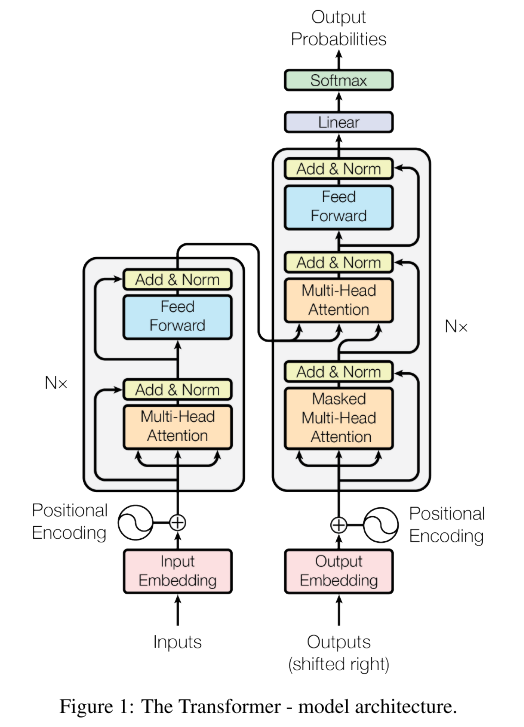
\includegraphics[width=\textwidth,height=\textheight,keepaspectratio]{mh_att.png}

\end{center}
\end{frame}


\begin{frame}[fragile]{The Transformer}
\begin{center}
	\begin{itemize}
		\item In “encoder-decoder attention” layers, the queries come from the previous decoder layer, and the memory keys and values come from the output of the encoder.
		\item Allows every position in the decoder to attend over all positions in the input sequence.
		\item Encoder has self-attention layers - Q,K,V come from same place. : Output of previous layer in the Encoder
		\item Decoder also has self-attention layers - allows each position in the decoder to attend to all positions in the decoder up to and including that position.
		\item Preserver auto regressive [2] property - mask out (by setting to $ - \infty$) to all input values of Softmax corresponding to illegal positions.
	\end{itemize}
[2] A. Graves, “Generating Sequences With Recurrent Neural Networks,” pp. 1–43.
\end{center}
\end{frame}

\begin{frame}[fragile]{Position-wise Feed-Forward Networks}
In addition to attention sub-layers, each of the layers in our encoder and decoder contains a fully connected feed-forward network - applied to each position separately and identically.

$$FFN(x) = max(0, x W_{1} + b_{1}) W_{2} + b_{2}$$

Weights are shared across positions, not across layers. [4]

[4] O. Press and L. Wolf, “Using the Output Embedding to Improve Language Models,” Aug. 2016.
\end{frame}

\begin{frame}[fragile]{Learning rate scheduling}
Adam optimizer with $\beta_{1} = 0.9$ and $\beta_{2} = 0.98$ and $\epsilon = 10^{-9}$

Varied learning rate over training time according to:
$$lrate = d_{model}^{-0.5} \times min(step\_num^{-0.5}, step\_num \times warmup\_steps^{-1.5})$$
\end{frame}


\begin{frame}[fragile]{Positional Encoding}
\begin{center}
	\begin{itemize}
		\item Transformer contains no Recurrence or Convolution
		\item We have to inject some information about the relative or absolute position
		\item Added at the bottom of both encoder and decoder
		\item same dimension ($d_{model}$) as the embeddings, so they can be summed
		\item Many choices of positional encoding - learned or fixed (ConvS2S [5])
	\end{itemize}
	$$PE_{(pos, 2_{i})} = sin(pos/1000^{2i/d_{model}})$$
	$$PE_{(pos, 2_{i+1})} = cos(pos/1000^{2i/d_{model}})$$
	
	[5] J. Gehring, M. Auli, D. Grangier, D. Yarats, and Y. N. Dauphin, “Convolutional Sequence to Sequence Learning,” May 2017.
\end{center}
\end{frame}

\begin{frame}[fragile]{Positional Encoding}
 \begin{itemize}
 	\item Each dimension of the positional encoding corresponds to a sinusoid
 	\item The wavelengths form a geometric progression from $2\pi$ to $10000 . 2\pi$
 	\item Hypothesis of the authors : allows the model to easily learn to attend by relative positions
 	\item  for any fixed offset $k$ $PE_{pos+k}$ can be represented as a linear function of $PE_{pos}$
 \end{itemize}
\end{frame}


\begin{frame}[fragile]{Positional Encoding - Example}
	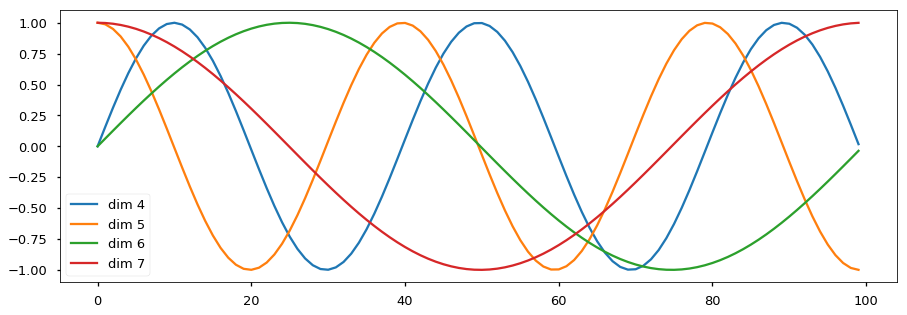
\includegraphics[width=\textwidth,height=\textheight,keepaspectratio]{pos_enc2.png}
	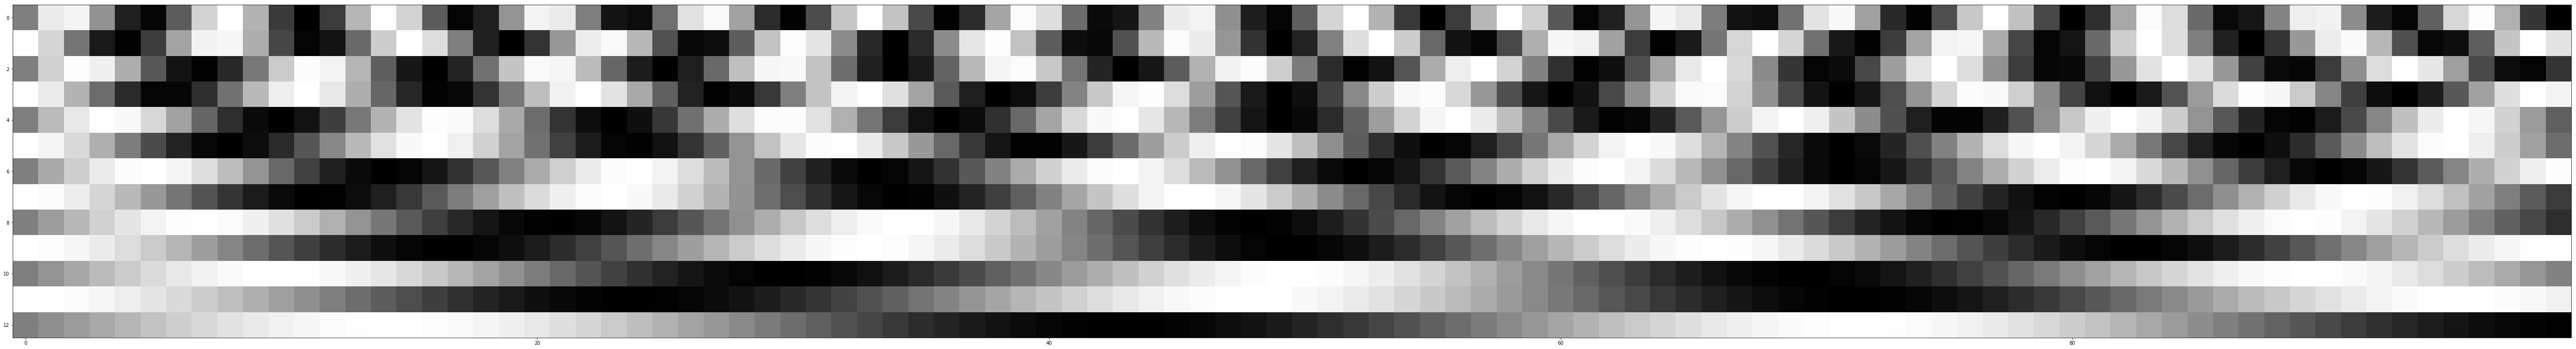
\includegraphics[width=\textwidth,height=\textheight,keepaspectratio]{pos_enc.png}
\end{frame}



\begin{frame}[fragile]{Other variants}
\begin{itemize}
	\item MultiHead Additive Attention - Replace dot product by sum and an MLP
	\item MultiHead locatiob aware attebtuib - Consider attention weights from previous positions and use a CNN (like Location aware Attention we discussed)
	\item MultiHead Multi Resolution Attention - Use different filter size for each head!
\end{itemize}
\end{frame}


{\setbeamercolor{palette primary}{fg=black, bg=yellow}
	\begin{frame}[standout]
	Thank you for your Attention.\\
	Questions?
\end{frame}
}

\end{document}